\documentclass[tikz,border=2pt]{standalone}
% Preámbulo común de los diagramas TikZ (misma paleta y letra que las notas)
\usepackage[T1]{fontenc}\usepackage[utf8]{inputenc}
\usepackage{libertinus}\usepackage{libertinust1math}
\usepackage[defaultsans,scale=0.92]{lato}
\usepackage{amsmath,amssymb,bm}
\usepackage{tikz}\usetikzlibrary{calc,positioning,arrows.meta,shapes.geometric,decorations.pathreplacing,decorations.pathmorphing,fit,backgrounds}
\definecolor{snlazul}{HTML}{1E5AA8}\definecolor{snlnoche}{HTML}{14213D}\definecolor{snlvioleta}{HTML}{6C4AB6}
\definecolor{snlcoral}{HTML}{D1495B}\definecolor{snlambar}{HTML}{E09F3E}\definecolor{snlverde}{HTML}{2A9D8F}
\definecolor{snlteal}{HTML}{0F7173}\definecolor{snlgris}{HTML}{5C677D}\definecolor{snlfondo}{HTML}{F4F6FA}
\tikzset{>={Stealth[length=2.2mm]},
  bloque/.style={draw=#1,fill=#1!8,thick,rounded corners=2pt,minimum height=11mm,minimum width=20mm,align=center,font=\small},
  bloque/.default=snlazul,
  suma/.style={draw=snlnoche,thick,circle,inner sep=0pt,minimum size=5mm},
  flecha/.style={->,thick,draw=snlnoche},
  etq/.style={font=\small,text=snlnoche},
  nota/.style={font=\footnotesize\sffamily,text=snlgris,align=center}}

\begin{document}
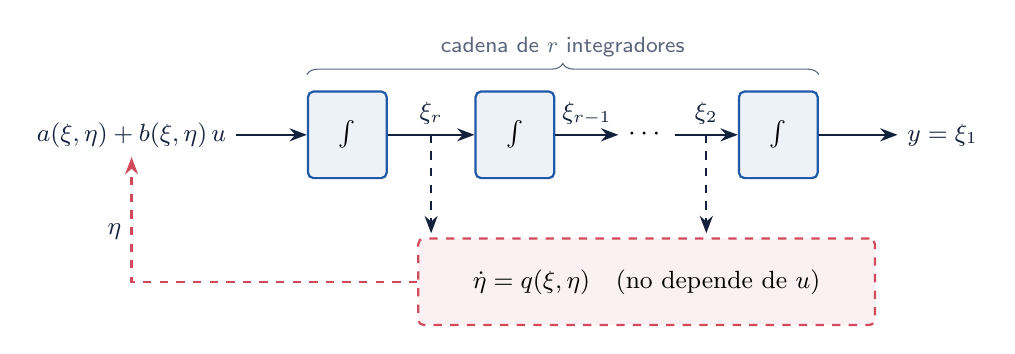
\begin{tikzpicture}
 \node[etq] (v) {$a(\xi,\eta)+b(\xi,\eta)\,u$};
 \node[bloque=snlazul,right=9mm of v,minimum width=10mm] (i1) {$\int$};
 \node[bloque=snlazul,right=11mm of i1,minimum width=10mm] (i2) {$\int$};
 \node[right=8mm of i2] (dots) {$\cdots$};
 \node[bloque=snlazul,right=8mm of dots,minimum width=10mm] (i3) {$\int$};
 \node[etq,right=10mm of i3] (y) {$y=\xi_1$};
 \draw[flecha] (v) -- (i1);
 \draw[flecha] (i1) -- node[above,etq]{$\xi_r$} (i2);
 \draw[flecha] (i2) -- node[above,etq]{$\xi_{r-1}$} (dots);
 \draw[flecha] (dots) -- node[above,etq]{$\xi_2$} (i3);
 \draw[flecha] (i3) -- (y);
 \node[bloque=snlcoral,dashed,below=11mm of dots,minimum width=58mm] (eta) {$\dot\eta=q(\xi,\eta)$\quad (no depende de $u$)};
 \draw[flecha,dashed] ($(i1.east)!0.5!(i2.west)$) -- ($(i1.east)!0.5!(i2.west)+(0,-12.5mm)$);
 \draw[flecha,dashed] ($(dots.east)!0.5!(i3.west)$) -- ($(dots.east)!0.5!(i3.west)+(0,-12.5mm)$);
 \draw[flecha,dashed,snlcoral] (eta.west) -| node[pos=0.7,left,etq]{$\eta$} (v.south);
 \draw[decorate,decoration={brace,amplitude=4pt},snlgris] (i1.north west)++(0,2mm) -- ($(i3.north east)+(0,2mm)$) node[midway,above=3pt,nota] {cadena de $r$ integradores};
\end{tikzpicture}
\end{document}
